\section{The Large Hadron Collider}
\label{sec:lhc}
Protons are delivered to the LHC by means of multiple intermediate accelerators: the Lineac2, the Proton Synchrotron Booster, the Proton Synchrotron (PS), and the Super Protron Synchrotron (SPS).
The PS was the first circular particle accelerator built at CERN in the late 1950s. 
In its current implementation the PS takes protons that originate in the Lineac2 linear accelerator at $50$ MeV that are then accelerated in the Proton Synchrotron Booster to $1.4$ GeV.
The protons are fed from the PS to the SPS which was commissioned in 1976 and has served to accelerate protons, antiprotons, electrons and positrons for various accelerators over its history.
Most notably the SPS accelerator provided the proton-antiproton beams that were used for the UA1 and UA2 experiments that accomplished the discovery of the $W$ and $Z$ bosons.
The SPS later provided the $e^{+}e^{-}$ beams that were used for LEP.
The two proton beams for the LHC are accelerated to their injection energy of $450$ GeV in the SPS at which point the radio-frequency resonating cavities of the LHC accelerate the beams to their collision energies.
A diagram of the CERN accelerator complex is shown in Figure \ref{fig:lhc}
\begin{figure*}[htpb]
\begin{center}
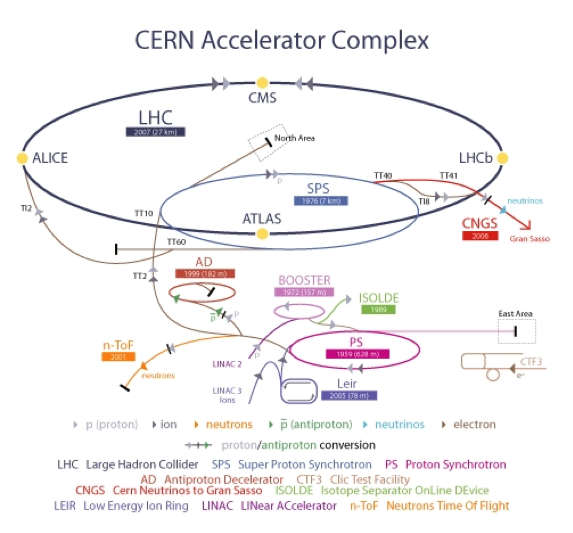
\includegraphics[width=0.85\textwidth]{plots/lhc.png}
\caption{Schematic of the CERN accelerator complex including intermediate accelerators that deliver the proton beams used in the LHC.}
\label{fig:lhc}
\end{center}
\end{figure*}

The proton is a composite particle, which in addition to having three ``valence'' quarks contains more sub-structure in the form of virtual quarks and gluons. 
In Section \ref{sec:qcd} it was shown that gluons interact with both themselves and quarks, thus the gluons that hold the proton together are responsible for producing quark-antiquark pairs which exist inside the proton.
The individual components, or partons, of the proton will each carry some fraction of the total momentum of the proton which is given by the parton distribution function (pdf) and is dependent on the energy of the proton.
In a hadron collision it is in fact the partons that produce the interaction rather that the proton itself.
The pdfs give the probability of finding a particular parton with longitudinal momentum fraction $x$ at a given momentum $Q$. 
Two example pdfs are shown in Figure \ref{fig:pdf}, one for low $Q$ and one for high $Q$.
Upon examination of Figure \ref{fig:pdf} one can see that as the energy of the proton increases, so too does the fraction of the momentum carried by the gluons.
At the energy of the LHC the pdf of the proton is dominated by gluons. 
%In comparison to the LHC, at the energy of the Tevatron the quarks carry a larger fraction of the momentum.
%For this reason colliding protons at the LHC would be somewhat equivalent to colliding protons and antiprotons, as it is more often that the interactions observed are provided by interacting gluons.
At the energy of the LHC, the dominance of the gluon in the pdf means that the majority of interactions are due to two gluons. 
Thus, there is little advantage in colliding protons and anti-protons.
This combined with the fact that antiprotons are difficult to produce and store leads to the conclusion that a proton-proton collider at the LHC energy scale is the logical choice.
\begin{figure*}[htpb]
\begin{center}
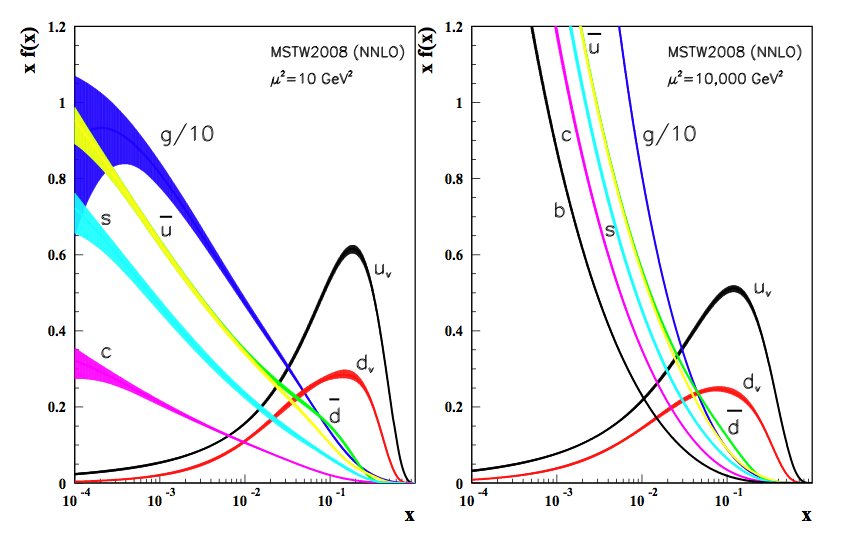
\includegraphics[width=0.85\textwidth]{plots/pdf.png}
\caption{Distributions of $x$ times the parton fraction $f(x)$ for the constituents of the proton at $Q^{2} = 10$ GeV$^{2}$ (left) and $Q^{2} = 10,000$ GeV$^{2}$\cite{PDGREVIEW}.}
\label{fig:pdf}
\end{center}
\end{figure*}


The collision of two protons rather than protons and antiprotons, while negating the difficulty of producing and storing antiprotons, leads to other difficulties.
The colliding particles now have the same charge and as such cannot share the same steering magnets. 
Two separate beam pipes and magnet systems must be used to steer the protons around the LHC ring in different directions.
An additional difficulty at the LHC is the energy at which the protons must be collided in order to probe new physics.
In order to steer the proton beams at an energy of $7$ TeV, dipole magnets are used which must be capable of providing greater than $8$ T magnetic fields.
The superconducting dipole magnets are made of \ce{NbTi} cables that are cooled to superfluid temperatures of $\sim2$ K.
An important aspect of superconducting magnets is quenching, or the process by which the magnet returns to a normal resistive state.
Quenching can occur due to heat dissipation inside the magnet.
A quench can be induced by increasing the current of the magnet, and as a result heat dissipation in the magnet will raise the temperature beyond the critical temperature of the material.
Upon re-energizing the magnet, a greater field can be achieved before a quench occurs, this process is referred to as a training quench.
Due to the number of training quenches required to bend the proton beams at their full $7$ TeV energy, it was decided to operate the accelerator with proton beams of $3.5$ TeV during the 2010 and 2011 data collection periods.
The data collection period of 2012 will see the beam energy increase to $8$ TeV, with the beam increasing to the design energy some time after the maintenance period of 2013-2014.

The magnitude of the Higgs signal to that of common QCD multi-jet events was shown in Section \ref{sec:history}, and similar situations exist for other new physics signals.
%The relative production rates of new physics and the QCD multi-jet processes is what drives the desire to operate the LHC at very high instantaneous luminosities.
In order to probe these rare processes a large number of interactions must be produced in order to collect statistically significant samples, thus the drive for very high integrated luminosities is demonstrated.
During the 2010 data collection period a total integrated luminosity of $36$ pb$^{-1}$ was collected, while during the 2011 data collection period a total integrated luminosity of $4.6$ fb$^{-1}$ was collected.
The integrated luminosity of the 2012 data collection period is projected to be in the range of $15$-$20$ fb$^{-1}$.
The schedule for the increase in luminosity at the LHC is enumerated in Table \ref{tab:lhcluminosity}.
In order to achieve a high luminosity, protons are grouped into high density ``bunches'' made up of multiple protons that are accelerated around the LHC ring. 
By bunching the protons together the probability of two protons having a hard scatter, or collision, is increased.
The luminosity can then be increased by increasing the number of protons in each bunch, thus increasing the number of interacting protons per collision, $N_{1}$ and $N_{2}$ for either beam.
The luminosity can further be increased by placing a larger number of bunches ($n$) in the LHC ring leading to a higher collision rate.
Finally the cross sectional area ($A$) of the beam is minimized at the collision points to maximize the probability of a collision. 
These three factors can be seen in the following equation that gives the instantaneous luminosity,
\begin{equation}
\Lagr = fn\frac{N_{1}N_{2}}{A}.
\end{equation}
A side effect of increasing the luminosity in this way is that while increasing the probability of an interesting collision, the probability of ``uninteresting'' collisions is also increased.
In fact it is common for multiple interactions to occur in the same bunch, up to $\sim 35$ in some cases for the 2011 data collection.
This presents a challenge to an analysis performed at a hadron collider in that each event contains an effective ``pile-up'' of multiple events that must be taken into account when searching for new physics.

\begin{table}[htpb]
\begin{center}
\caption{LHC LUMINOSITY INCREASE SCHEDULE}
\begin{tabular}{lc}
\toprule
Year & Integrated Luminosity [fb$^{-1}$] \\
\midrule
2010 & $0.036$ \\
2011 & $4.6$ \\
2012 & $15$-$20$(projected) \\
\bottomrule
\end{tabular}
\label{tab:lhcluminosity}
\end{center}
\end{table}
% magnets
% proton-proton
% luminosity

